\chapter[Análise dos Resultados]{Análise dos Resultados}\label{ch:analiseResultados}
  Este capítulo tem como objetivo discutir  os resultados obtidos durante a realização dos testes. Dentre estes
resultados, estão presentes as fontes de erros levantadas com a experiência do desenvolvimento,
suas respectivas correções, dentro do possível, e a análise dos resultados da utilização do
sistema no contexto da reabilitação motora. Desse modo, este
capítulo está dividido nas seções: Casos de testes funcionais (\ref{sec:testes}),
Fontes de erro (\ref{sol:fontesErro}), Outros resultados (\ref{sol:outrosResultados}), Análise dos resultados (\ref{sol:viabilidade}) e Problemas enfrentados (\ref{ch:problemas}).

\section{Casos de testes funcionais}\label{sec:testes}
  O principal objetivo dos casos de testes funcionais, é a observação e a análise do sistema. Após a realização de todos os casos de testes propostos, foi possível chegar a
uma análise dos resultados da utilização do sistema no contexto da reabilitação motora,
 a qual será apresentada na seção \ref{sol:viabilidade}.

 Os casos de testes funcionais consistem em cinco situações, nas quais a solução foi analisada,
variando entre elas o movimento e ambiente. Buscando analisar os resultados obtidos em cada contexto.

  Os dados obtidos em cada caso de teste está estruturado de acordo com a tabela \ref{tab:analise}.

  \begin{table}[H]
  \centering
  \caption{Estruturação dos Dados}
  \label{tab:analise}
  \begin{tabular}{@{}|l|l|l|l|@{}}
  \toprule
  \textbf{Movimento} & \textbf{Complexidade} & \textbf{Luz ambiente} & \textbf{exatidão} \\ \bottomrule
  \end{tabular}
  \end{table}

\begin{itemize}
  \item \textbf{Movimento}: O nome e descrição do movimento análisado, \textbf{exemplo}: Levantar e abaixar braço direito.
  \item \textbf{Complexidade}: Essa variável é referente a complexidade da execução do movimento, para o mapeamento do \textit{kinect} e acompanhamento do usuário.
   A rotulação dessa variável segue a tabela \ref{tab:compl}.

    \begin{table}[H]
    \centering
    \caption{Rotulação da complexidade do Movimento}
    \label{tab:compl}
    \begin{tabular}{@{}|c|c|@{}}
\toprule
\textbf{Complexidade} & \textbf{Descrição}                                                                                                                                          \\ \midrule
\textbf{Alta}         & \begin{tabular}[c]{@{}c@{}}Execução do movimento é de difícil mapeamento para \\ o kinect e para acompanhamento do usuário.\end{tabular}                    \\ \midrule
\textbf{Media}        & \begin{tabular}[c]{@{}c@{}}Execução do movimento é de dificuldade moderada para\\ o mapeamento para o kinect e para acompanhamento do usuário.\end{tabular} \\ \midrule
\textbf{Baixa}        & \begin{tabular}[c]{@{}c@{}}Execução do movimento é de dificuldade baixa para\\  o mapeamento para o kinect e para acompanhamento do usuário.\end{tabular}   \\ \bottomrule
\end{tabular}
\end{table}

  \item \textbf{Luz ambiente}: Com a premissa básica de um ambiente com pelo menos um metro e meio do sensor, essa variável diz respeito
a intensidade da luminosidade do ambiente, podendo ser \textbf{boa}, \textbf{regular} e \textbf{ruim}.

  \item \textbf{Exatidão}: Essa variável é referente a exatidão que o \textit{kinect} acompanha e corrige o movimento do usuário.
   A rotulação dessa variável segue a tabela \ref{tab:compl}.
    \begin{table}[H]
    \centering
    \caption{Rotulação da complexidade do Movimento}
    \label{tab:compl}
    \begin{tabular}{@{}|c|c|@{}}
\toprule
\textbf{Exatidão} & \textbf{Descrição}                                                                                                        \\ \midrule
\textbf{Boa}      & \begin{tabular}[c]{@{}c@{}}Bom acompanhamento e correção no movimento\\  executado pelo usuário\end{tabular}              \\ \midrule
\textbf{Regular}  & \begin{tabular}[c]{@{}c@{}}Regular acompanhamento e correção no movimento\\  executado pelo usuário.\end{tabular}         \\ \midrule
\textbf{Ruim}     & \begin{tabular}[c]{@{}c@{}}Ruim ou péssimo acompanhamento e correção no movimento\\  executado pelo usuário.\end{tabular} \\ \bottomrule
\end{tabular}
\end{table}

\end{itemize}


  As próximas seções apresentam os casos de testes funcionais com diferentes variáveis, possibilitando a ánalise do comportamento do sistema em tais
  casos. Todos os testes foram feitos em um ambiente com quatro metros quadrados e o sensor \textit{kinect} em uma altura de aproximadamente um metro e meio.

\subsection{Levantar braço direito}\label{sub:teste1}
  Os resultados obtidos com o caso de teste estão dispostos na tabela \ref{tab:teste1}. Esse caso de teste consiste no levantamento do braço direito, em uma velocidade
  baixa.

\subsubsection{Relatório de teste}\label{sub:relteste1}
Como pode ser observado na tabela \ref{tab:teste1} que a luz ambiente tem grande influência no mapeamento do \textit{kinect}. Podemos
observar na imagem \ref{img:teste1}, o esqueleto à esquerda é o movimento
que está sendo executado pelo usuário, assim o movimento tem que ser executado
com certa fidelidade, caso contrário os erros serão apresentados na forma de esferas sobre as juntas que se devem ser corrigidas. E na imagem \ref{img2:teste1} a correta execução do movimento.

\begin{table}[H]
\centering
\caption{Teste 1}
\label{tab:teste1}
\begin{tabular}{@{}|c|c|l|l|l|@{}}
\toprule
\multicolumn{1}{|l|}{ } & \multicolumn{1}{l|}{\textbf{Movimento}} & \textbf{Complexidade} & \textbf{Luz Ambiente} & \textbf{Exatidão} \\ \midrule
1                                 & Levantar Braço Dir.                     & Baixa                 & Boa                   & Boa               \\ \midrule
2                                 & Levantar Braço Dir.                     & Baixa                 & Regular               & Regular           \\ \midrule
3                                 & Levantar Braço Dir.                     & Baixa                 & Ruim                  & Ruim              \\ \bottomrule
\end{tabular}
\end{table}


\begin{figure}[H]
\centering
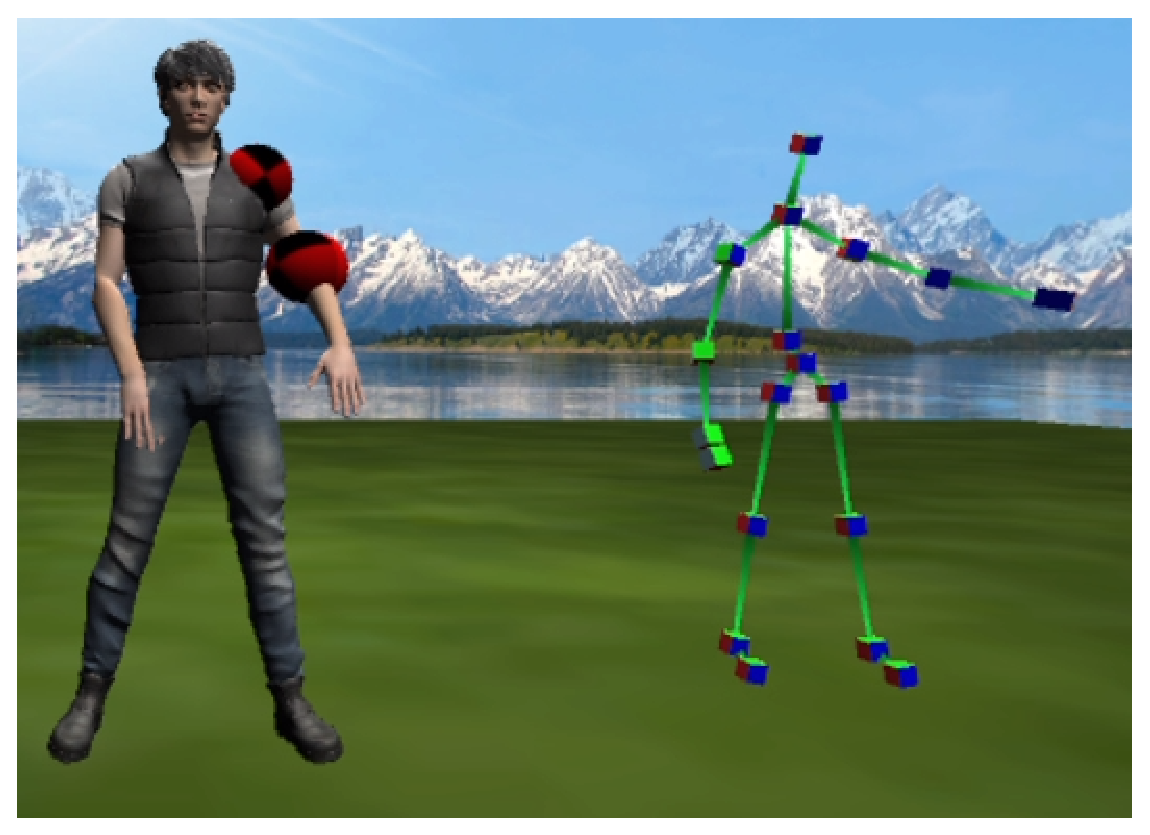
\includegraphics [keepaspectratio=true,scale=0.60]{figuras/img2teste1.eps}
\caption{Movimento com presença de falhas}
\label{img:teste1}
\end{figure}

\begin{figure}[H]
\centering
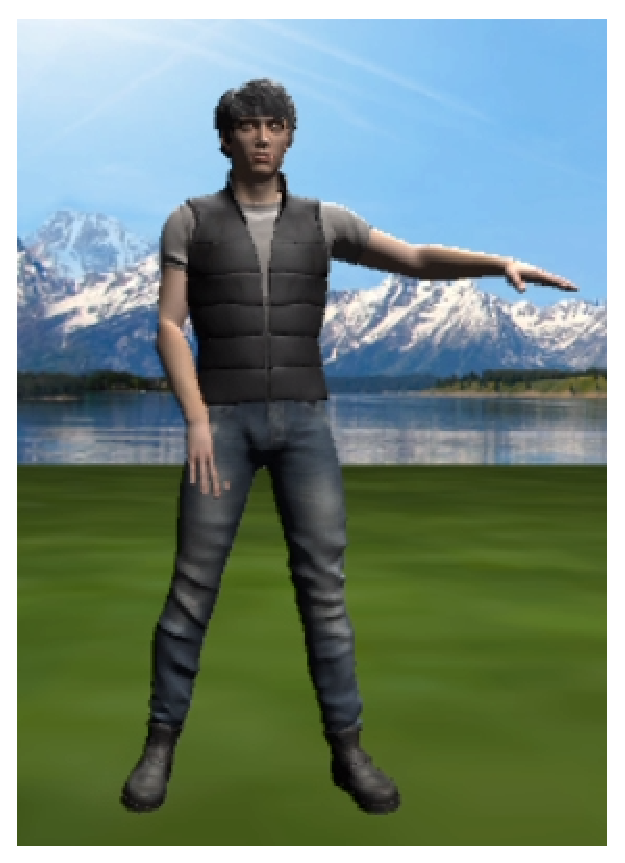
\includegraphics [keepaspectratio=true,scale=0.60]{figuras/imgteste1.eps}
\caption{Movimento correto}
\label{img2:teste1}
\end{figure}


\subsection{Levantar dois braços}\label{sub:teste2}
Os resultados obtidos com o teste estão dispostos na tabela \ref{tab:teste2}. Esse teste consiste no levantamento dos dois braços , em uma velocidade
baixa.

\subsubsection{Relatório de teste}\label{sub:relteste2}

Como pode ser observado na tabela \ref{tab:teste2} a luz ambiente tem grande influência no mapeamento do \textit{kinect}, porém com uma luz ambiente boa
a exatidão do sensor é \textbf{boa}.

\begin{table}[H]
\centering
\caption{Teste 2}
\label{tab:teste2}
\begin{tabular}{@{}|c|c|l|l|l|@{}}
\toprule
\multicolumn{1}{|l|}{ } & \multicolumn{1}{l|}{\textbf{Movimento}} & \textbf{Complexidade} & \textbf{Luz Ambiente} & \textbf{Exatidão} \\ \midrule
1                                 & Levantar os  Braços                     & Baixa                 & Boa                   & Boa               \\ \midrule
2                                 & Levantar os  Braços                     & Baixa                 & Regular               & Regular           \\ \midrule
3                                 & Levantar os  Braços                     & Baixa                 & Ruim                  & Ruim              \\ \bottomrule
\end{tabular}
\end{table}


\subsection{Sentar e levantar em uma cadeira de lado para o sensor}\label{sub:teste3}
Os resultados obtidos com o teste estão dispostos na tabela \ref{tab:teste3}. Esse teste consiste em sentar e levantar em uma cadeira de lado ao \textit{kinect}, em uma velocidade
baixa.

\subsubsection{Relatório de teste}\label{sub:relteste3}
Como pode ser observado na tabela \ref{tab:teste3} o \textit{kinect} não consegue rastrear uma pessoa de lado, o sensor se perde nas referências mostrando isntabilidade como pode ser
visto na imagem \ref{img:teste3}.


\begin{table}[H]
\centering
\caption{Teste 3}
\label{tab:teste3}
\begin{tabular}{@{}|c|c|l|l|l|@{}}
\toprule
\multicolumn{1}{|l|}{ } & \multicolumn{1}{l|}{\textbf{Movimento}} & \textbf{Complexidade} & \textbf{Luz Ambiente} & \textbf{Exatidão} \\ \midrule
1                                 & Sentar de lado em Cadeira                     & Alta                 & Boa                   & Ruim               \\ \midrule
2                                 & Sentar de lado em Cadeira                     & Alta                 & Regular               & Ruim           \\ \midrule
3                                 & Sentar de lado em Cadeira                     & Alta                 & Ruim                  & Ruim              \\ \bottomrule
\end{tabular}
\end{table}

\begin{figure}[H]
\centering
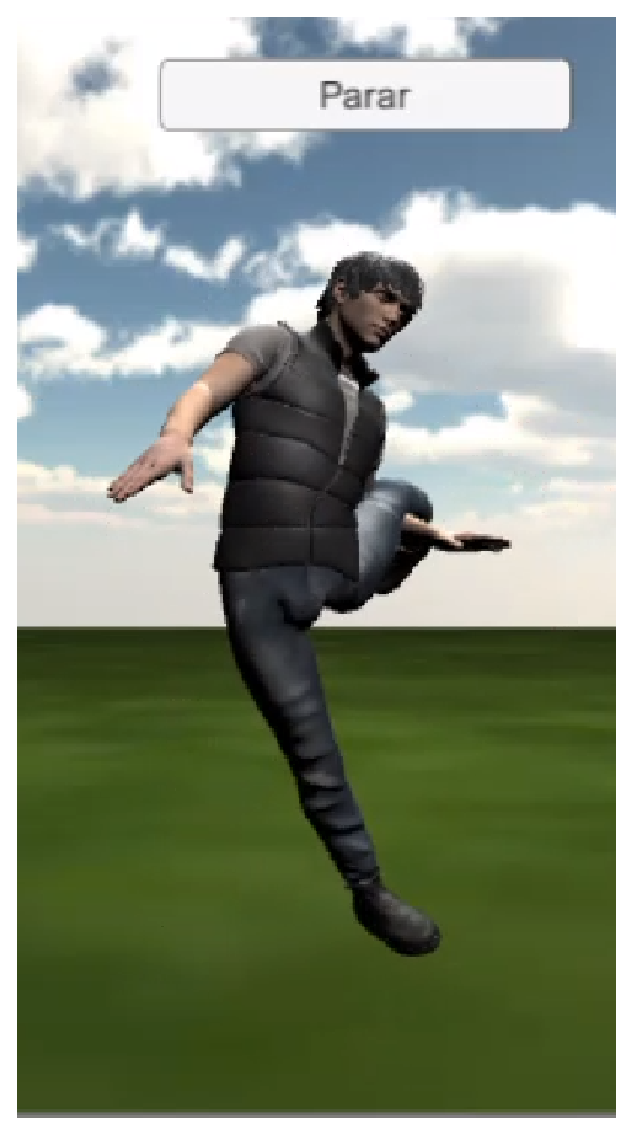
\includegraphics [keepaspectratio=true,scale=0.60]{figuras/cadeira.eps}
\caption{Instabilidade com o usário sentando de lado em uma cadeira}
\label{img:teste3}
\end{figure}

\subsection{Sentar e levantar em uma cadeira de frente para o sensor}\label{sub:teste4}
Os resultados obtidos com o teste estão dispostos na tabela \ref{tab:teste4}. Esse teste consiste em sentar e levantar em uma cadeira de frente ao \textit{kinect} , em uma velocidade
baixa.

\subsubsection{Relatório de teste}\label{sub:relteste4}
Como pode ser observado na tabela \ref{tab:teste4} o \textit{kinect} não conseguiu rastrear o movimento da pessoa sentando em uma cadeira. O sensor se perde nas referências das juntas
sobrepostas, mostrando instabilidade como pode ser visto na imagem \ref{img:teste4}.

\begin{table}[H]
\centering
\caption{Teste 4}
\label{tab:teste4}
\begin{tabular}{@{}|c|c|l|l|l|@{}}
\toprule
\multicolumn{1}{|l|}{ } & \multicolumn{1}{l|}{\textbf{Movimento}} & \textbf{Complexidade} & \textbf{Luz Ambiente} & \textbf{Exatidão} \\ \midrule
1                                 & Sentar de frente em Cadeira                     & Alta                 & Boa                   & Ruim               \\ \midrule
2                                 & Sentar de frente em Cadeira                     & Alta                 & Regular               & Ruim           \\ \midrule
3                                 & Sentar de frente em Cadeira                     & Alta                 & Ruim                  & Ruim              \\ \bottomrule
\end{tabular}
\end{table}


\begin{figure}[H]
\centering
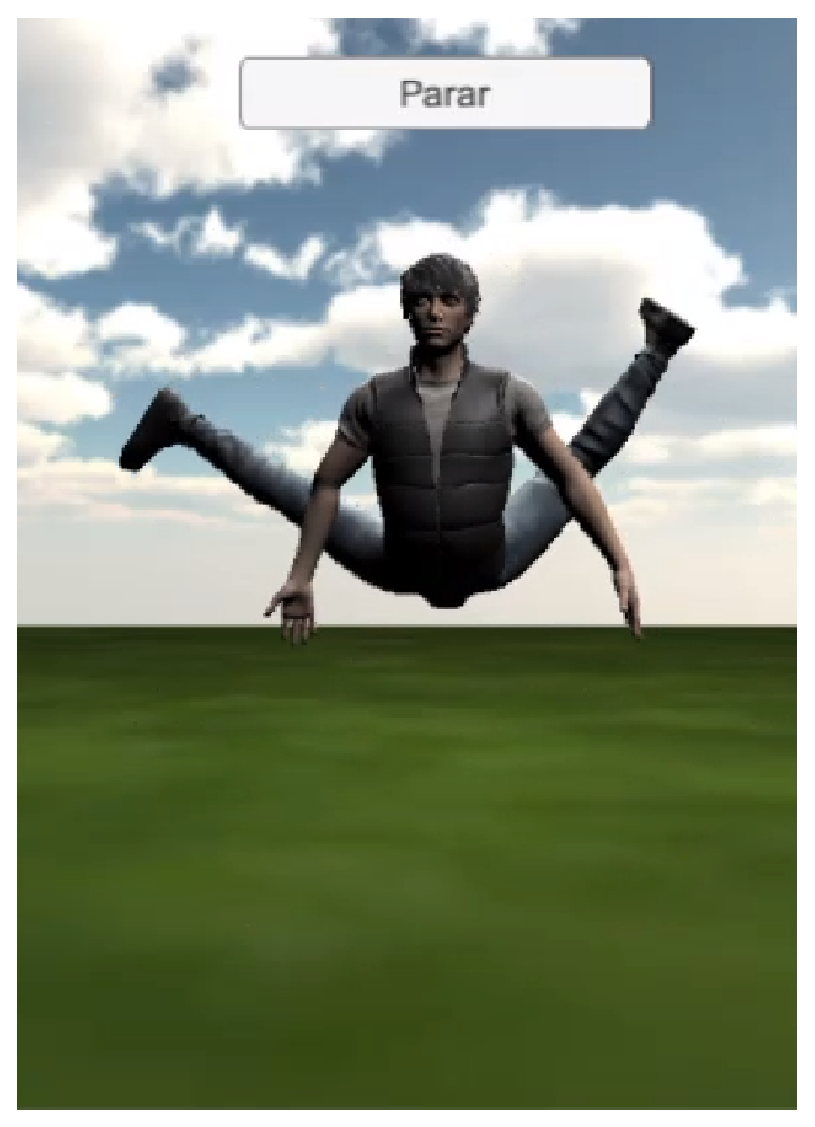
\includegraphics [keepaspectratio=true,scale=0.60]{figuras/cadeiraFrente.eps}
\caption{Instabilidade com o usuário sentando de frente em uma cadeira}
\label{img:teste4}
\end{figure}

\subsection{Agachamento}\label{sub:teste5}
Os resultados obtidos com o teste estão dispostos na tabela \ref{tab:teste5}. Esse teste consiste no usuário agachar-se em uma velocidade
baixa.

\subsubsection{Relatório de teste}\label{sub:relteste2}
Como pode ser observado na tabela \ref{tab:teste4} o \textit{kinect} não conseguiu rastrear muito bem o movimento. O sensor se perde nas referências das juntas
sobrepostas, mostrando instabilidade como pode ser visto na imagem \ref{img:teste5}.

\begin{table}[H]
\centering
\caption{Teste 5}
\label{tab:teste5}
\begin{tabular}{@{}|c|c|l|l|l|@{}}
\toprule
\multicolumn{1}{|l|}{ } & \multicolumn{1}{l|}{\textbf{Movimento}} & \textbf{Complexidade} & \textbf{Luz Ambiente} & \textbf{Exatidão} \\ \midrule
1                                 & Agachar                     & Alta                 & Boa                   & Regular               \\ \midrule
2                                 & Agachar                     & Alta                 & Regular               & Ruim           \\ \midrule
3                                 & Agachar                     & Alta                 & Ruim                  & Ruim              \\ \bottomrule
\end{tabular}
\end{table}


\begin{figure}[H]
\centering
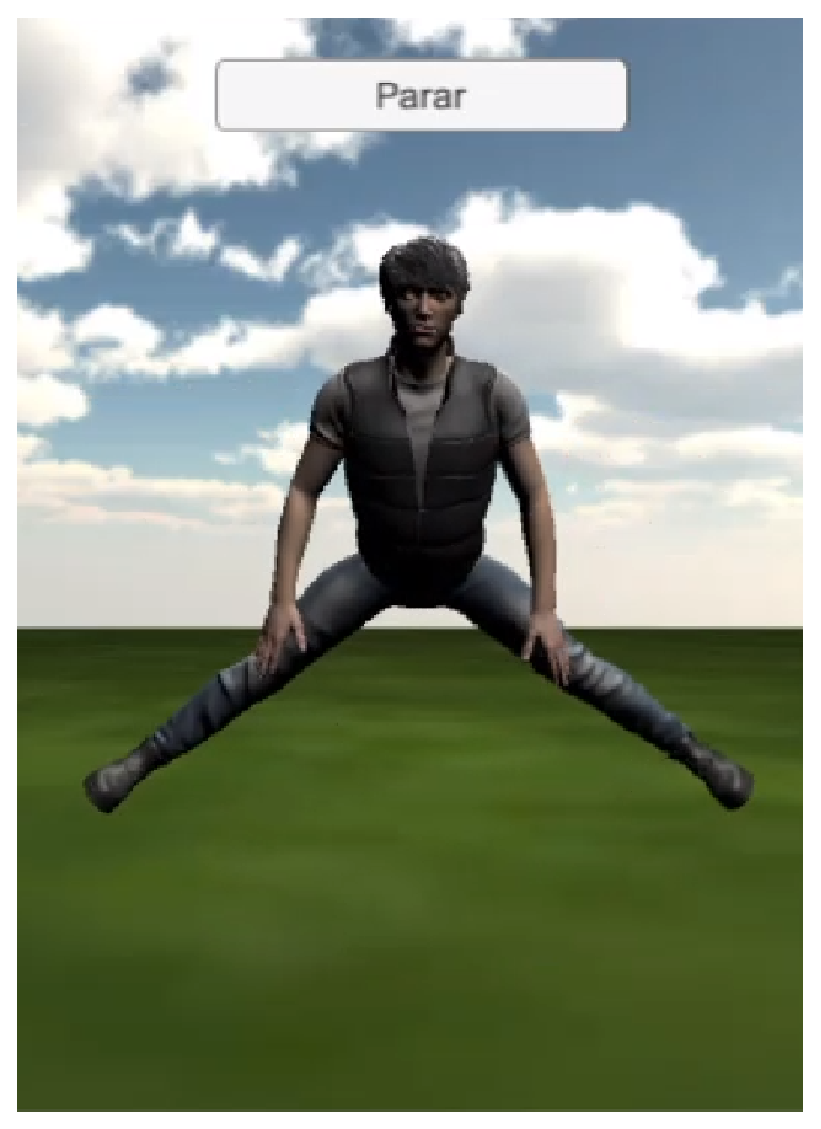
\includegraphics [keepaspectratio=true,scale=0.60]{figuras/agachar.eps}
\caption{Pouca fidelidade com o real movimento}
\label{img:teste5}
\end{figure}


\section{Casos de testes funcionais por junta}\label{sec:testes}
  O principal objetivo dos casos de testes funcionais por junta, é a observação e a análise de cada junta que o \textit{kinect} é capaz de rastrear, podendo validar
  o comportamento do sistema para cada junta. Previamente devemos estar cientes que não é possível isolar o comportamento de cada junta, dado que não é possível separá-las
  do corpo, sendo assim, alguns casos de testes serão responsáveis pela análise de mais de uma junta.

  \subsection{Cabeça}\label{sub:cabeca}
  Os resultados obtidos com o teste estão dispostos na tabela \ref{tab:cabeca}. Esse teste consiste no usuário movimentar a cabeça para os lados. Esse movimento
  foi gravado previamente e serão apresentados as imagens referentes a comparação.

  \subsubsection{Relatório de teste}\label{sub:cabeca}
  Como pode ser observado na tabela \ref{tab:cabeca} o movimento foi corrigido com exatidão, dada as limitações de luz ambiente. O sistema corrige o usuário quando este
  não está fazendo o movimento correto da cabeça como pode ser visto em \ref{img:cabecaErrada} e não apresenta nenhum erro quando o movimento está sendo executado
  corretamente como pode ser visto em \ref{img:cabecaCerta}

  \begin{table}[H]
  \centering
  \caption{Teste de junta referente a cabeça}
  \label{tab:cabeca}
  \begin{tabular}{@{}|c|c|l|l|l|@{}}
  \toprule
  \multicolumn{1}{|l|}{ } & \multicolumn{1}{l|}{\textbf{Movimento}} & \textbf{Complexidade} & \textbf{Luz Ambiente} & \textbf{Exatidão} \\ \midrule
  1                                 & Cabeça                     & Baixa                 & Boa                   & Boa               \\ \midrule
  2                                 & Cabeça                     & Baixa                 & Regular               & Regular           \\ \midrule
  3                                 & Cabeça                     & Baixa                 & Ruim                  & Ruim              \\ \bottomrule
  \end{tabular}
  \end{table}

  \begin{figure}[H]
  \centering
  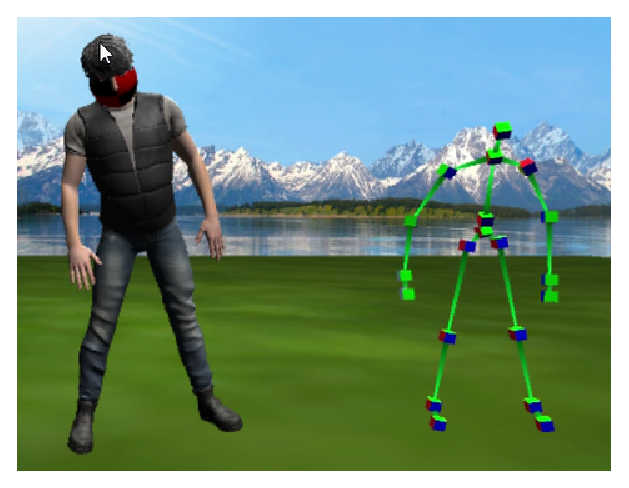
\includegraphics [keepaspectratio=true,scale=1]{figuras/cabecaErrada.eps}
  \caption{Movimento sendo exercitado de forma incorreta propositalmente para haver correção do sistema.}
  \label{img:cabecaErrada}
  \end{figure}

  \begin{figure}[H]
  \centering
  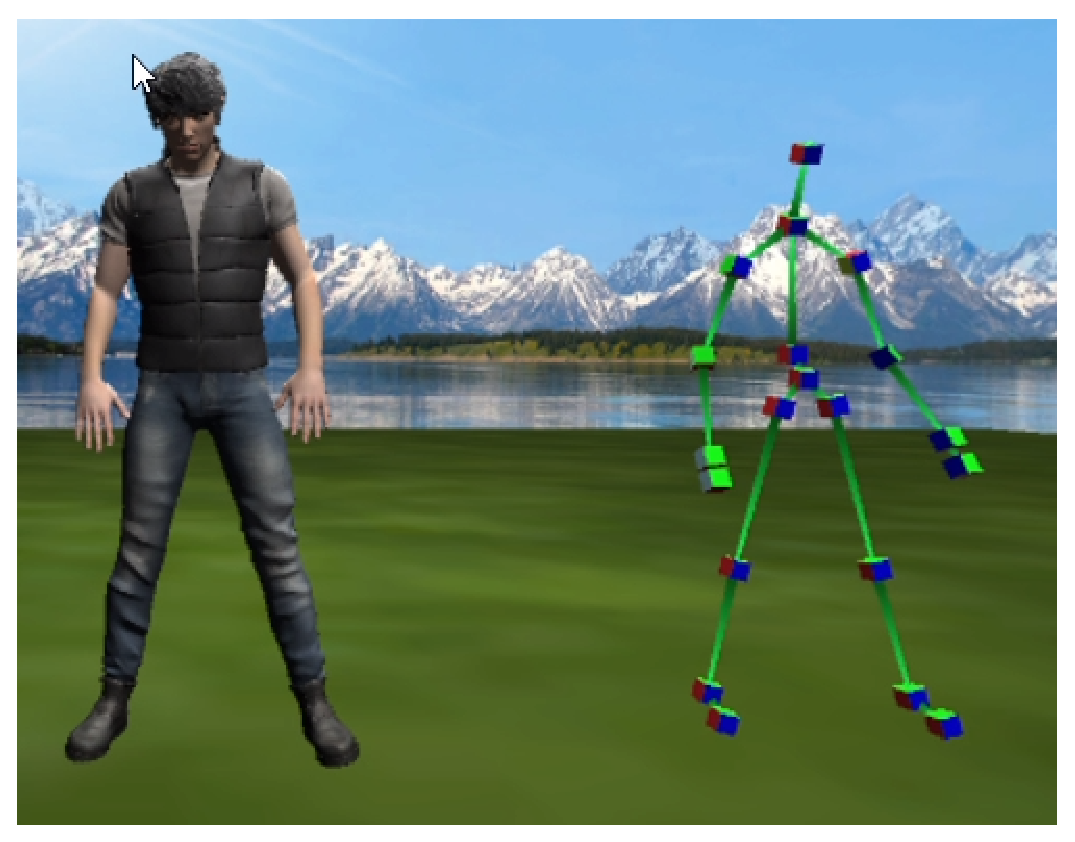
\includegraphics [keepaspectratio=true,scale=0.60]{figuras/cabecaCerta.eps}
  \caption{Movimento sendo exercitado de forma correta para não haver correção do sistema.}
  \label{img:cabecaCerta}
  \end{figure}


  \subsection{Coluna}\label{sub:coluna}
  Os resultados obtidos com o teste estão dispostos na tabela \ref{tab:coluna}. Esse teste consiste no usuário movimentar-se com o tronco para frente, diferente do movimento do avatar. Esse movimento
  foi gravado previamente e serão apresentados as imagens referentes a comparação.

  \subsubsection{Relatório de teste}\label{sub:coluna}
  Como pode ser observado na tabela \ref{tab:coluna} o movimento foi corrigido com exatidão, dada as limitações de luz ambiente. O sistema corrige o usuário quando este
  não está fazendo o movimento correto da coluna como pode ser visto em \ref{img:colunaErrada} e não apresenta nenhum erro quando o movimento está sendo executado
  corretamente como pode ser visto em \ref{img:colunaCerta}

  \begin{table}[H]
  \centering
  \caption{Teste de junta referente a cabeça}
  \label{tab:coluna}
  \begin{tabular}{@{}|c|c|l|l|l|@{}}
  \toprule
  \multicolumn{1}{|l|}{ } & \multicolumn{1}{l|}{\textbf{Movimento}} & \textbf{Complexidade} & \textbf{Luz Ambiente} & \textbf{Exatidão} \\ \midrule
  1                                 & Coluna                     & Baixa                 & Boa                   & Boa               \\ \midrule
  2                                 & Coluna                     & Baixa                 & Regular               & Regular           \\ \midrule
  3                                 & Coluna                     & Baixa                 & Ruim                  & Ruim              \\ \bottomrule
  \end{tabular}
  \end{table}

  \begin{figure}[H]
  \centering
  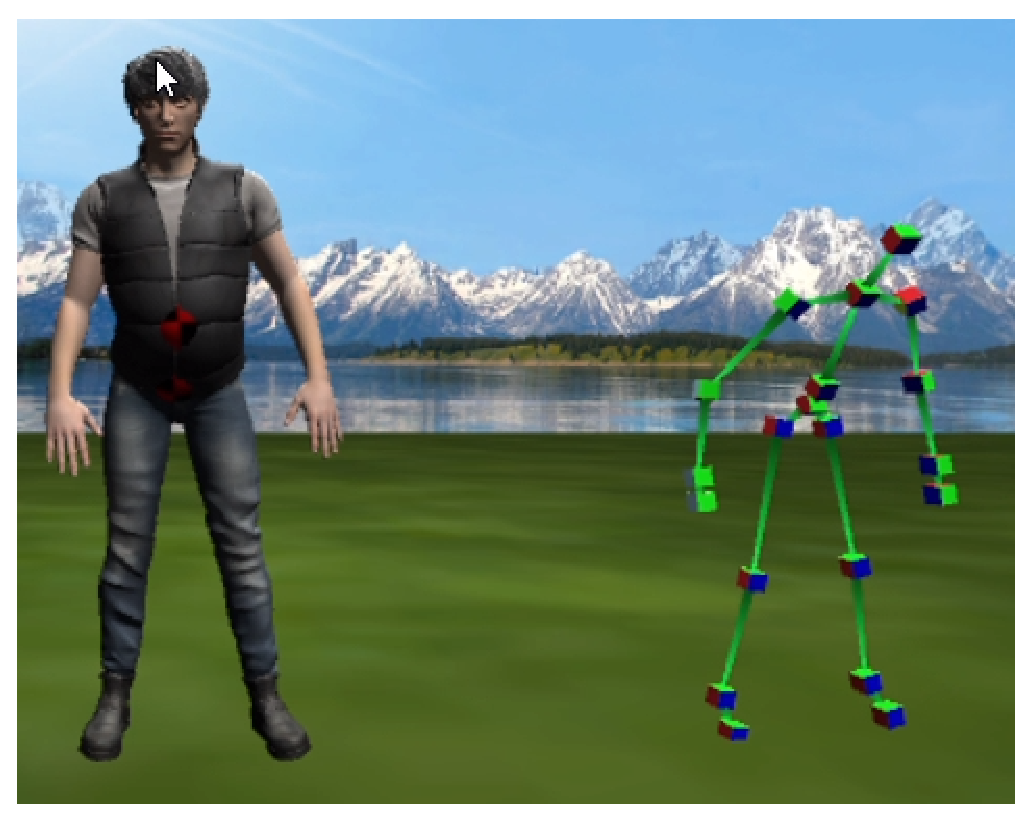
\includegraphics [keepaspectratio=true,scale=0.60]{figuras/colunaErrada.eps}
  \caption{Movimento sendo exercitado de forma incorreta propositalmente para haver correção do sistema.}
  \label{img:colunaErrada}
  \end{figure}

  \begin{figure}[H]
  \centering
  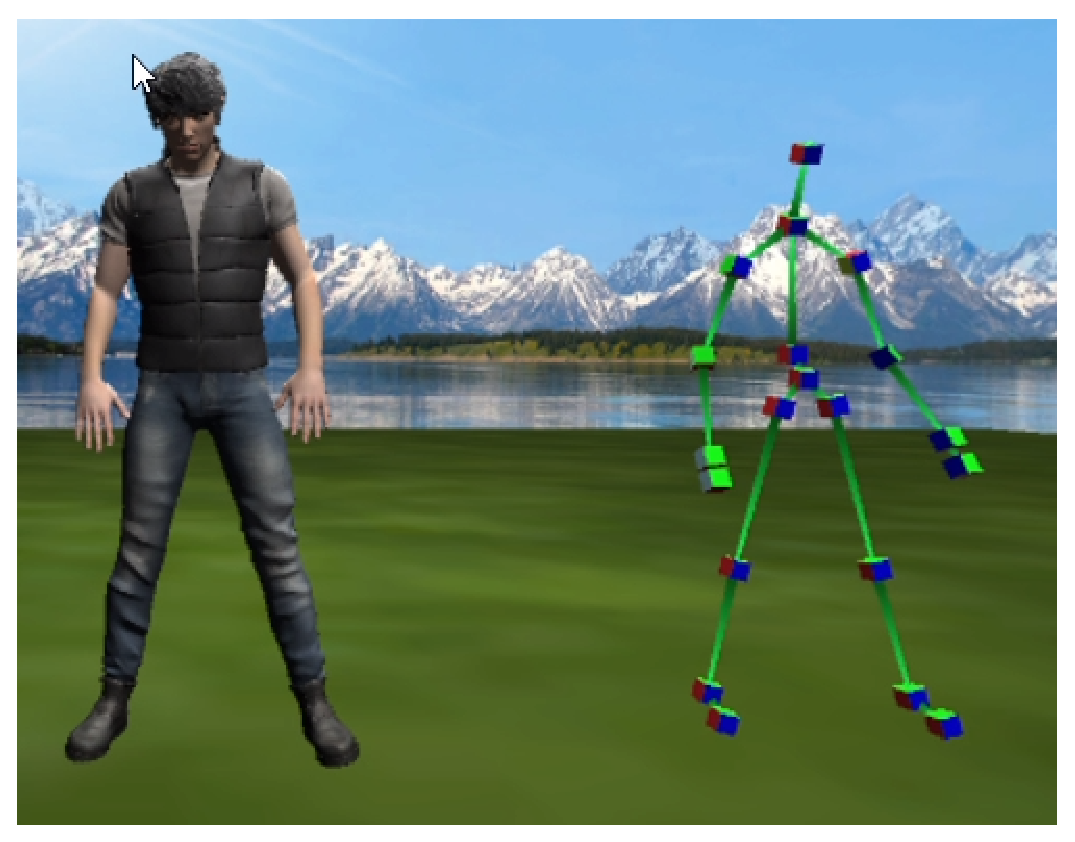
\includegraphics [keepaspectratio=true,scale=0.60]{figuras/cabecaCerta.eps}
  \caption{Movimento sendo exercitado de forma correta para não haver correção do sistema.}
  \label{img:colunaCerta}
  \end{figure}

  \subsection{Pernas}\label{sub:perna}
  Os resultados obtidos com o teste estão dispostos na tabela \ref{tab:perna}. Esse teste consiste na análise de várias juntas, sendo elas:
  \begin{itemize}
    \item Quadril direito;
    \item Joelho direito;
    \item Pé direito;
    \item Quadril esquerdo;
    \item Joelho esquerdo;
    \item Pé esquerdo;
  \end{itemize}

  O teste consiste em levantar a perna direita e esquerda, sendo que hora o usuário levantava, hora não.

  \subsubsection{Relatório de teste}\label{sub:perna}
  Como pode ser observado na tabela \ref{tab:perna} o movimento foi corrigido com exatidão, não tendo diferença entre os lados direito e esquerdo do corpo, dada as limitações de luz ambiente. O sistema corrige o usuário quando este
  não está fazendo o movimento correto da perna como pode ser visto nas imagens \ref{img:pernaEsquerdaErrada} e \ref{img:pernaDireitaErrada} e não apresenta nenhum erro quando o movimento está sendo executado
  corretamente como pode ser visto em \ref{img:pernaEsquerdaCerta} e  \ref{img:pernaDireitaCerta}.

  \begin{table}[H]
  \centering
  \caption{Teste de junta referente a cabeça}
  \label{tab:perna}
  \begin{tabular}{@{}|c|c|l|l|l|@{}}
  \toprule
  \multicolumn{1}{|l|}{ } & \multicolumn{1}{l|}{\textbf{Movimento}} & \textbf{Complexidade} & \textbf{Luz Ambiente} & \textbf{Exatidão} \\ \midrule
  1                                 & Quadris                     & Baixa                 & Boa                   & Boa               \\ \midrule
  2                                 & Quadris                     & Baixa                 & Regular               & Regular           \\ \midrule
  3                                 & Quadris                     & Baixa                 & Ruim                  & Ruim              \\ \bottomrule
  4                                 & Joelhos                     & Baixa                 & Boa                   & Boa               \\ \midrule
  5                                 & Joelhos                     & Baixa                 & Regular               & Regular           \\ \midrule
  6                                 & Joelhos                     & Baixa                 & Ruim                  & Ruim              \\ \bottomrule
  7                                 & Pés                         & Baixa                 & Boa                   & Boa               \\ \midrule
  8                                 & Pés                         & Baixa                 & Regular               & Regular           \\ \midrule
  9                                 & Pés                         & Baixa                 & Ruim                  & Ruim              \\ \bottomrule
  \end{tabular}
  \end{table}

  \begin{figure}[H]
  \centering
  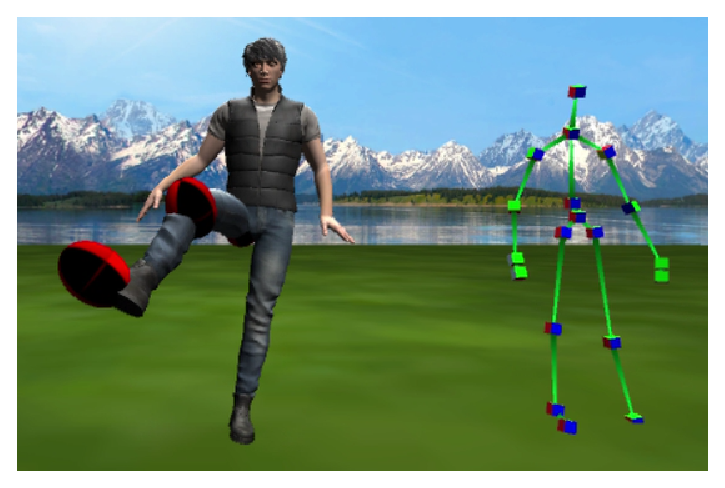
\includegraphics [keepaspectratio=true,scale=0.60]{figuras/pernaDireitaErrada.eps}
  \caption{Movimento sendo exercitado de forma incorreta propositalmente para haver correção do sistema.}
  \label{img:pernaDireitaErrada}
  \end{figure}

  \begin{figure}[H]
  \centering
  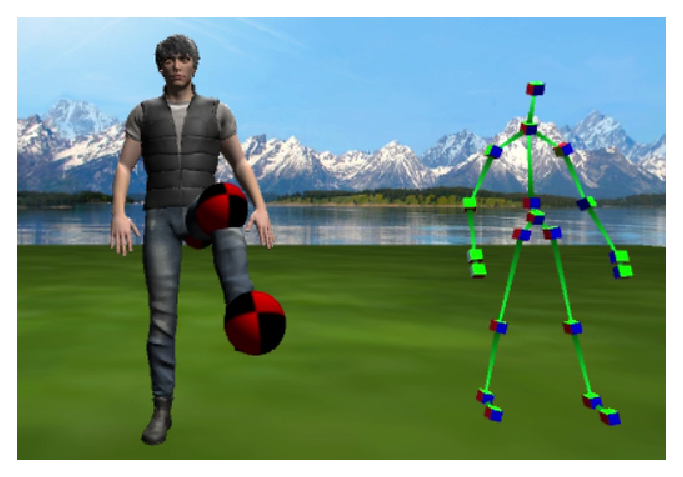
\includegraphics [keepaspectratio=true,scale=0.60]{figuras/pernaEsquerdaErrada.eps}
  \caption{Movimento sendo exercitado de forma incorreta propositalmente para haver correção do sistema.}
  \label{img:pernaEsquerdaErrada}
  \end{figure}


  \begin{figure}[H]
  \centering
  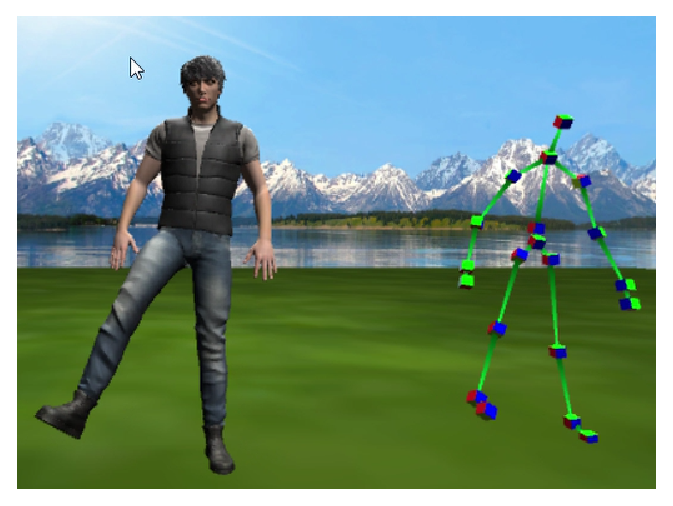
\includegraphics [keepaspectratio=true,scale=0.60]{figuras/pernaDireitaCerta.eps}
  \caption{Movimento sendo exercitado de forma correta para não haver correção do sistema.}
  \label{img:pernaDireitaCerta}
  \end{figure}

  \begin{figure}[H]
  \centering
  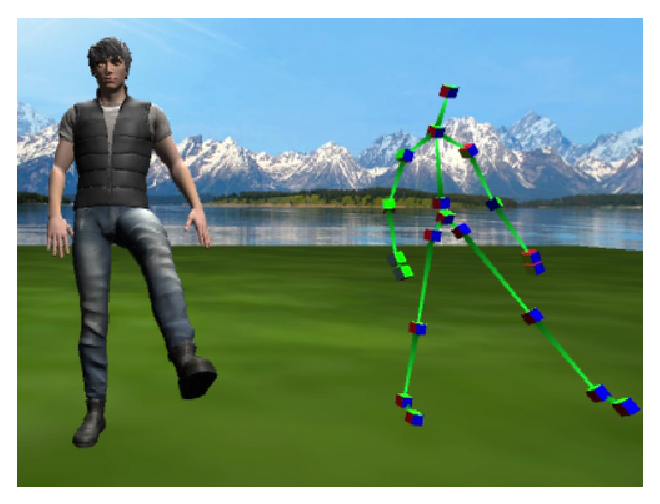
\includegraphics [keepaspectratio=true,scale=0.60]{figuras/pernaEsquerdaCerta.eps}
  \caption{Movimento sendo exercitado de forma correta para não haver correção do sistema.}
  \label{img:pernaEsquerdaCerta}
  \end{figure}


  \subsection{Braços}\label{sub:braco}
  Os resultados obtidos com o teste estão dispostos na tabela \ref{tab:braco}. Esse teste consiste na análise de várias juntas, sendo elas:
  \begin{itemize}
    \item Ombro direito;
    \item Cotovelo direito;
    \item Mão direito;
    \item Ombro esquerdo;
    \item Cotovelo esquerdo;
    \item Mão esquerdo;
  \end{itemize}

  O teste consiste em levantar a braço direito e esquerdo, sendo que hora o usuário levantava, hora não.

  \subsubsection{Relatório de teste}\label{sub:braco}
  Como pode ser observado na tabela \ref{tab:braco} o movimento foi corrigido com exatidão, não tendo diferença entre os lados direito e esquerdo do corpo, dada as limitações de luz ambiente. O sistema corrige o usuário quando este
  não está fazendo o movimento correto da braço como pode ser visto nas imagens \ref{img:bracoEsquerdaErrada} e \ref{img:bracoDireitaErrada} e não apresenta nenhum erro quando o movimento está sendo executado
  corretamente como pode ser visto em \ref{img:bracoEsquerdaCerta} e  \ref{img:bracoDireitaCerta}.

  \begin{table}[H]
  \centering
  \caption{Teste de junta referente ao braço}
  \label{tab:braco}
  \begin{tabular}{@{}|c|c|l|l|l|@{}}
  \toprule
  \multicolumn{1}{|l|}{ } & \multicolumn{1}{l|}{\textbf{Movimento}} & \textbf{Complexidade} & \textbf{Luz Ambiente} & \textbf{Exatidão} \\ \midrule
  1                                 & Ombros                     & Baixa                 & Boa                   & Boa               \\ \midrule
  2                                 & Ombros                     & Baixa                 & Regular               & Regular           \\ \midrule
  3                                 & Ombros                     & Baixa                 & Ruim                  & Ruim              \\ \bottomrule
  4                                 & Cotovelos                     & Baixa                 & Boa                   & Boa               \\ \midrule
  5                                 & Cotovelos                     & Baixa                 & Regular               & Regular           \\ \midrule
  6                                 & Cotovelos                     & Baixa                 & Ruim                  & Ruim              \\ \bottomrule
  7                                 & Mãos                         & Baixa                 & Boa                   & Boa               \\ \midrule
  8                                 & Mãos                         & Baixa                 & Regular               & Regular           \\ \midrule
  9                                 & Mãos                         & Baixa                 & Ruim                  & Ruim              \\ \bottomrule
  \end{tabular}
  \end{table}

  \begin{figure}[H]
  \centering
  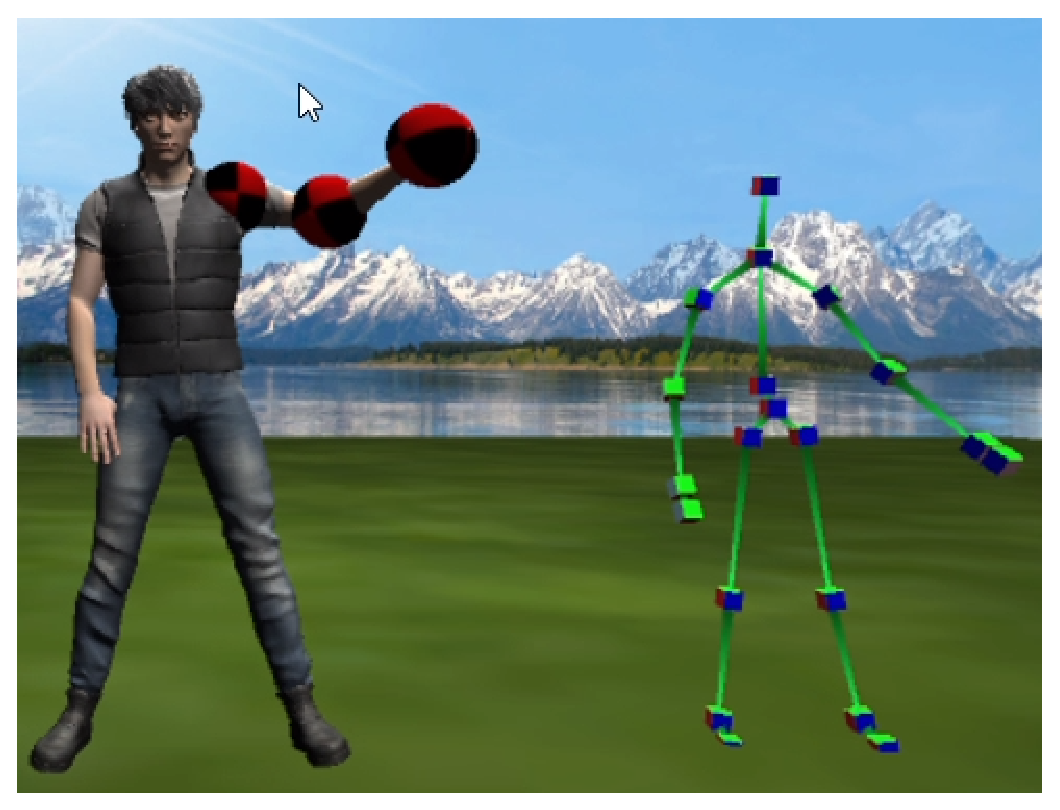
\includegraphics [keepaspectratio=true,scale=0.60]{figuras/bracoDireitaErrada.eps}
  \caption{Movimento sendo exercitado de forma incorreta propositalmente para haver correção do sistema.}
  \label{img:bracoDireitaErrada}
  \end{figure}

  \begin{figure}[H]
  \centering
  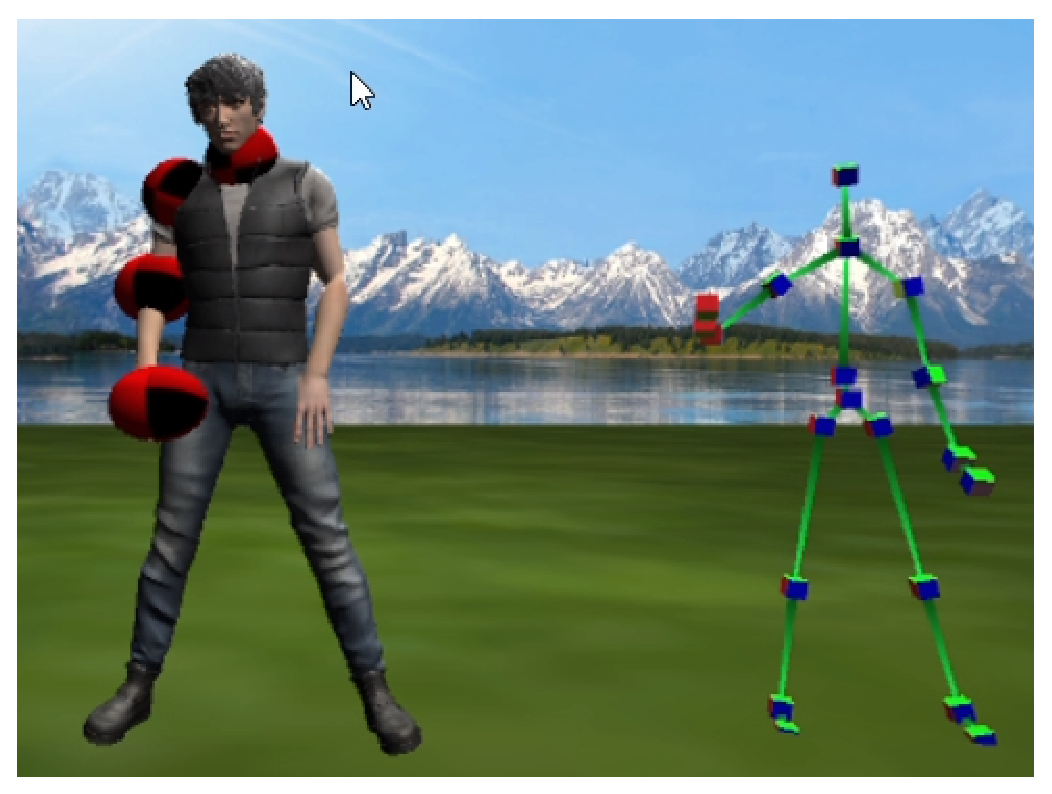
\includegraphics [keepaspectratio=true,scale=0.60]{figuras/bracoEsquerdaErrada.eps}
  \caption{Movimento sendo exercitado de forma incorreta propositalmente para haver correção do sistema.}
  \label{img:bracoEsquerdaErrada}
  \end{figure}


  \begin{figure}[H]
  \centering
  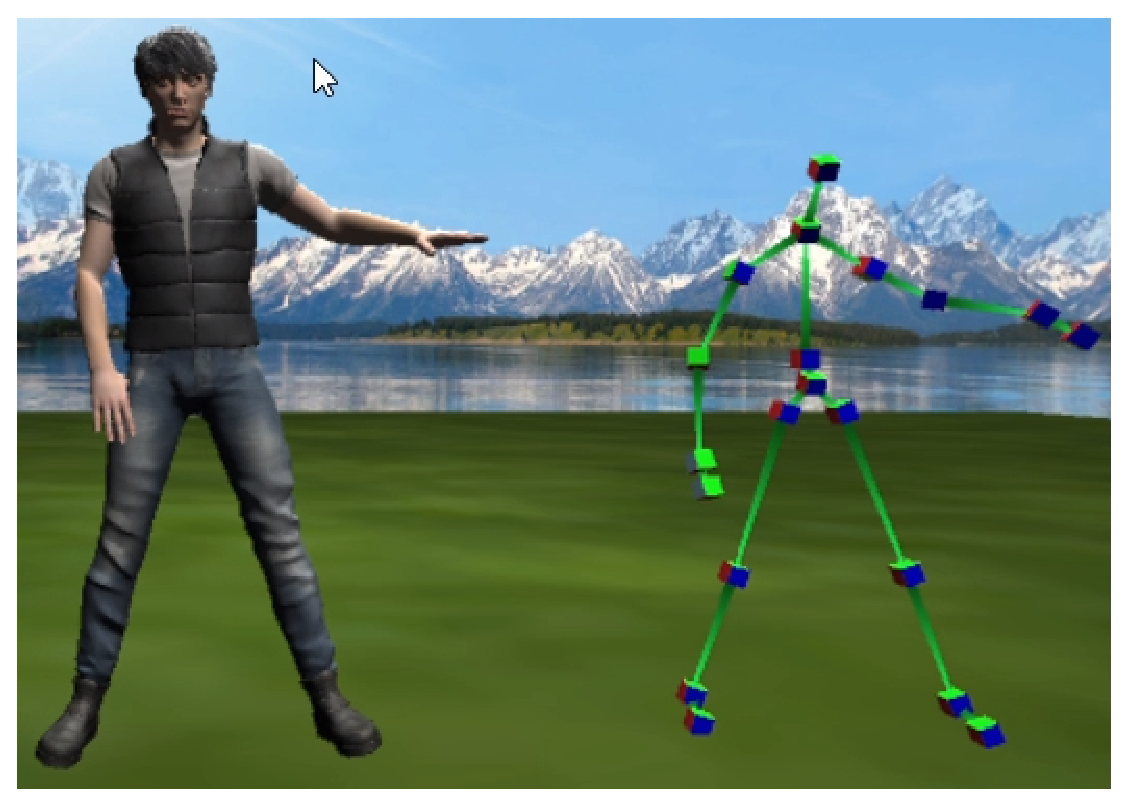
\includegraphics [keepaspectratio=true,scale=0.60]{figuras/bracoDireitaCerta.eps}
  \caption{Movimento sendo exercitado de forma correta para não haver correção do sistema.}
  \label{img:bracoDireitaCerta}
  \end{figure}

  \begin{figure}[H]
  \centering
  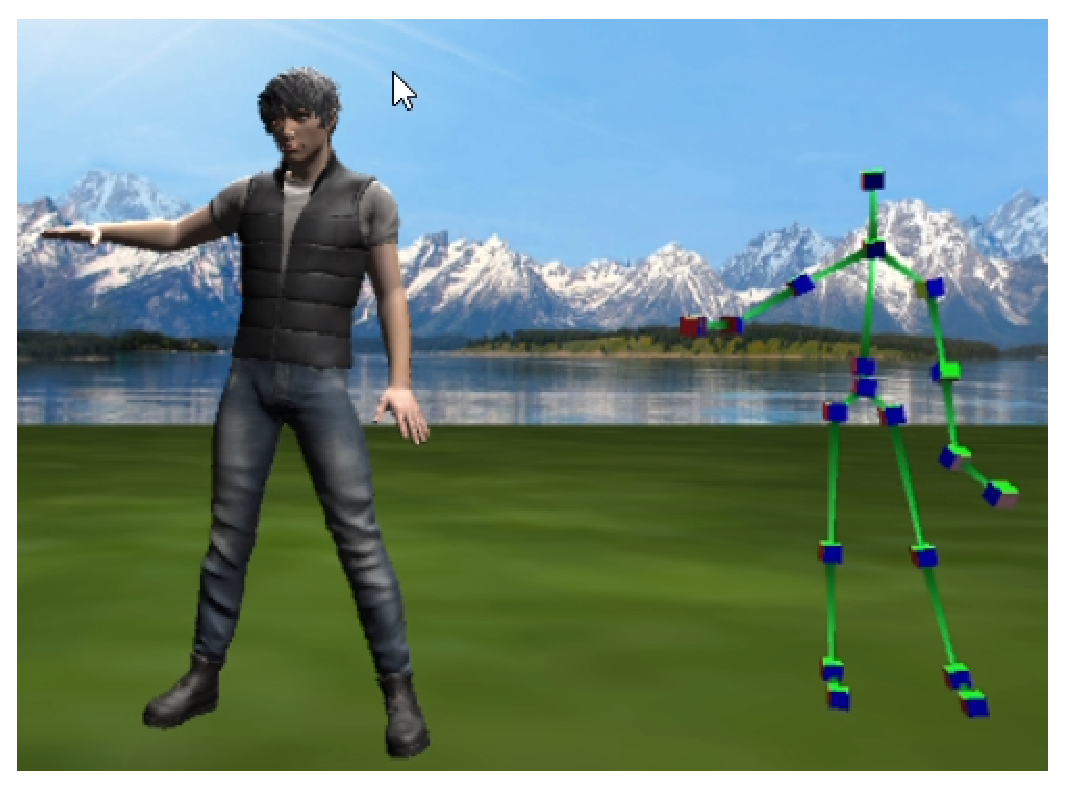
\includegraphics [keepaspectratio=true,scale=0.60]{figuras/bracoEsquerdaCerta.eps}
  \caption{Movimento sendo exercitado de forma correta para não haver correção do sistema.}
  \label{img:bracoEsquerdaCerta}
  \end{figure}





\section{Fontes de Erro}\label{sol:fontesErro}
  Como já mencionando anteriormente, a principal fonte do erro do sistema é devido as limitações do \textit{kinect}, seja pela precisão ou pela luz do ambiente.
Por este motivo, é aconselhavel que durante a execução dos movimentos, o ambiente esteja livre de possíveis interferências no mapeio do  sensor, além de estar bem iluminado. Quanto a precisão,
durante a realização do desenvolvimento buscou-se minimizar a margem de erro do sensor aumentando a tolerância angular sobre o movimento das juntas.

\section{Outros resultados}\label{sol:outrosResultados}
  Nesta seção é apresentada outros resultados obtidos ao decorrer do desenvolvimento deste trabalho.

\subsection{Arquitetura completa}\label{sol:arquiCompleta}
Em proposta apresentada na entrega do primeiro documento, foi apresentada a arquitetura completa, uma arquitetura de módulos, onde cada módulo é responsável
pelo comportamento de uma parte do sistema. Esta arquitetura se encontra em estado bem inicial, e foi desenvolvida
em python 3 \cite{pythondoc}. Nela temos 4 (quatro) módulos, sendo eles chamados de:

\begin{itemize}
  \item \textbf{Sensor}: Módulo responsável pelo comportamento do sensor;
  \item \textbf{Visualização}: Módulo responsável pelo comportamento e comunicação com a parte de visualização do avatar 3D;
  \item \textbf{Processamento}: Módulo responsável pelo comportamento de todo o processamento das informações das juntas;
  \item \textbf{Armazenamento}: Módulo responsável pelo compartamento de armazenar todas as informações do sistema.
\end{itemize}


Esta arquitetura é \textit{multiprocessing}, ou seja, cada módulo é executado em um processo diferente. Essa abordagem se explica pelo fato do algoritmo do
Baptista \cite{roberto}, ser em tempo real o que se trata de um processmento muito complexo, necessitanto-se de um processo dedicado. Esta implementação se encontra em estado bem inicial e pode ser encontrada \href{https://gitlab.com/ricardogtx/tcc2}{aqui} \footnote{https://gitlab.com/ricardogtx/tcc2} .

Abaixo mostramos um diagrama de sequências do sistema com essa arquitetura.

\begin{figure}[H]
\centering
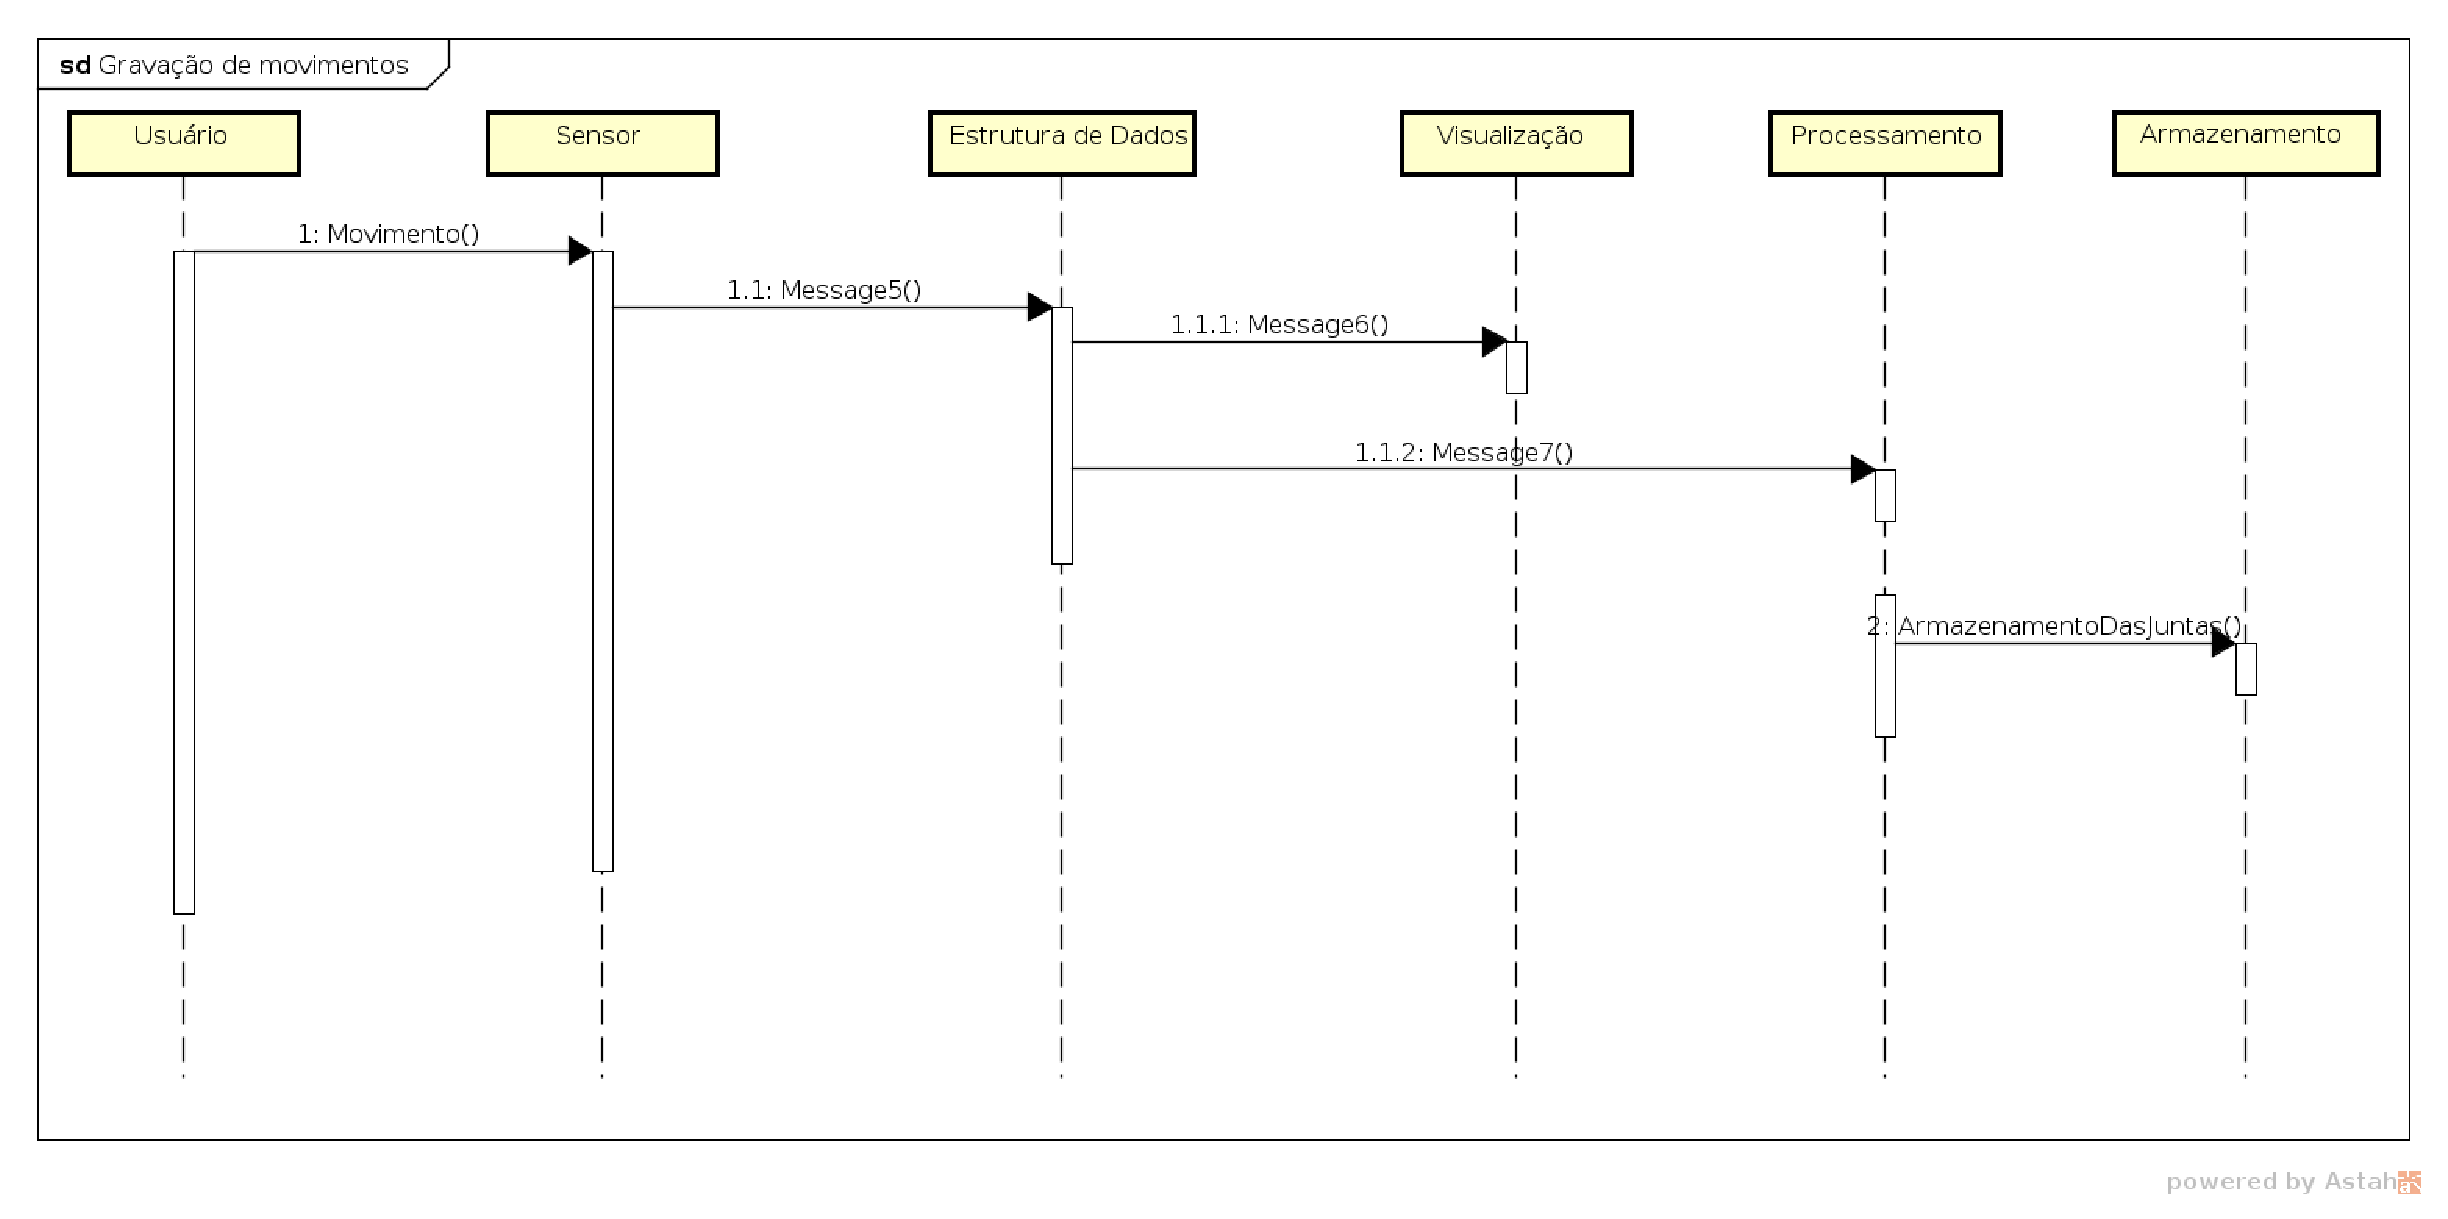
\includegraphics [keepaspectratio=true,scale=0.37]{figuras/dsPythonGravacao.eps}
\caption{Diagrama de sequência responsável pela troca das mensagens do sistema ao gravar um movimento.}
\label{img:dspythong}
\end{figure}

\begin{figure}[H]
\centering
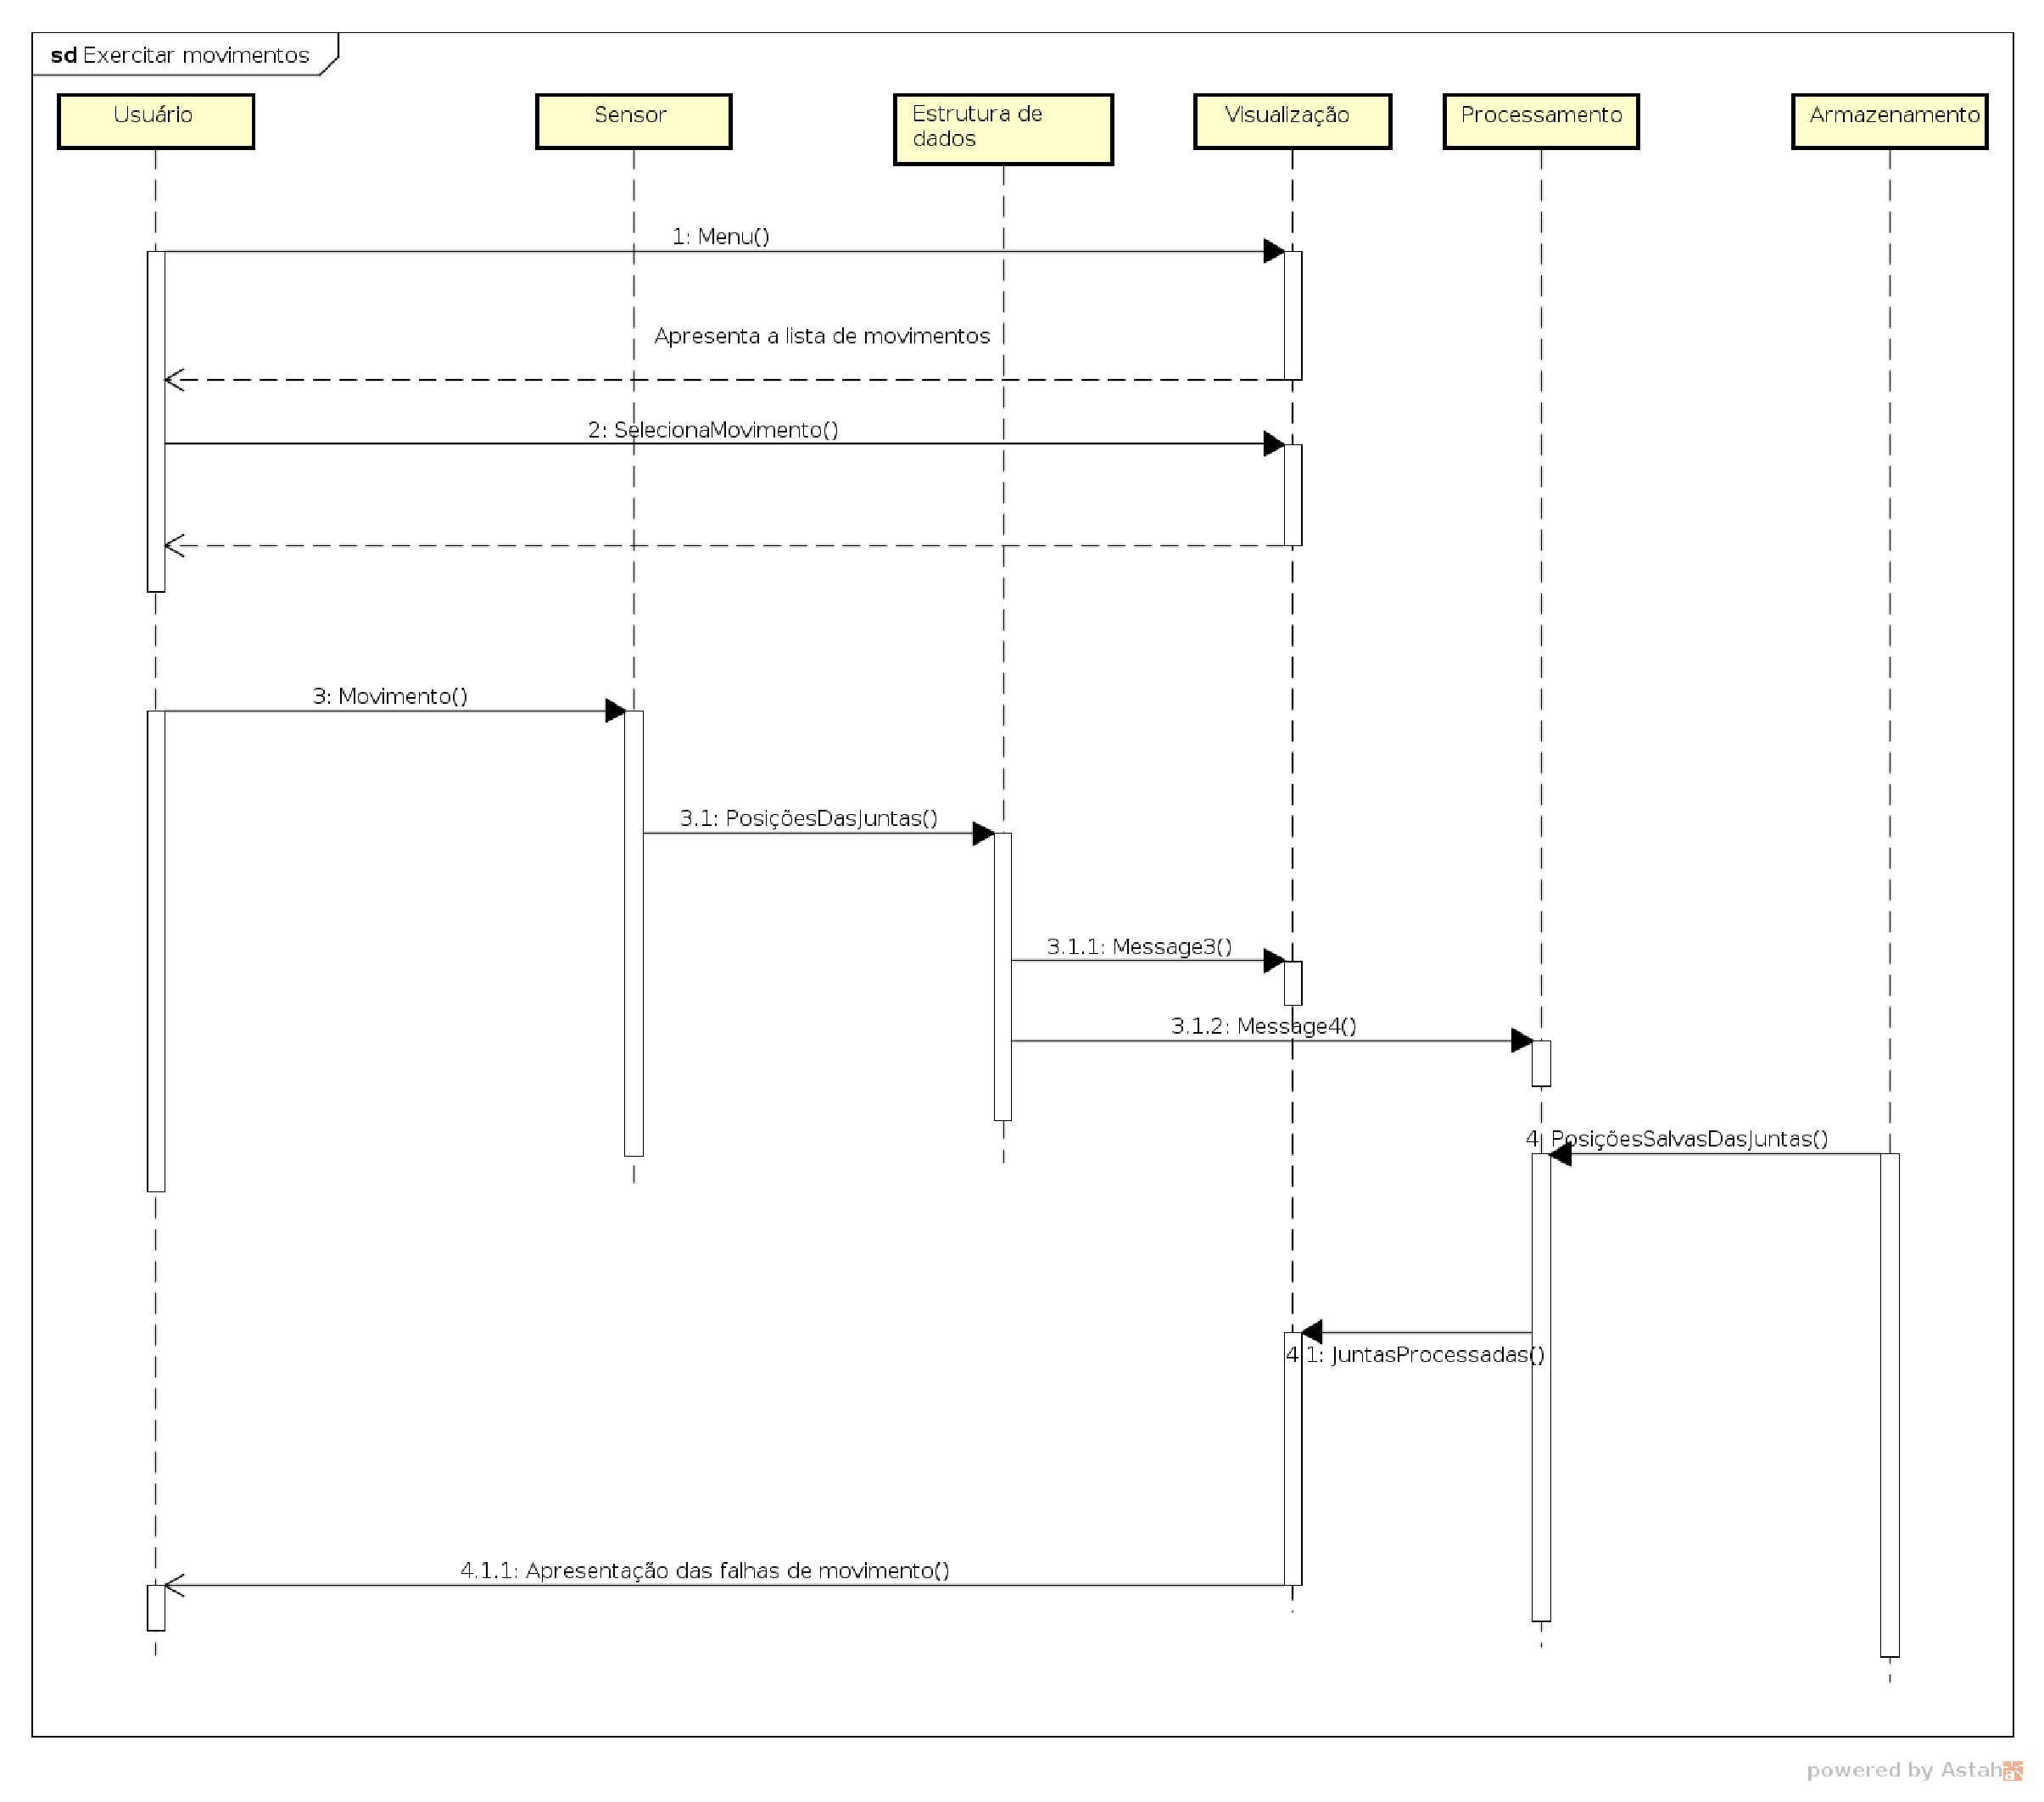
\includegraphics [keepaspectratio=true,scale=0.38]{figuras/dsPythonExecitar.eps}
\caption{Diagrama de sequência responsável pela troca das mensagens do sistema ao exercitar um movimento.}
\label{img:dspythone}
\end{figure}



 Essa abordagem não foi implementada por completo, devido ao nível de complexidade em se conseguir produzir um sistema com esses requisitos, no perído disponível para produção. Esta
 abordagem ficou enviável também, devido aos problemas encontrados durante o desenvolvimento deste trabalho, o que será mais explicado em \ref{ch:problemas}.


\section{Análise dos resultados}\label{sol:viabilidade}
Apesar da análise entre as juntas está sendo feita da maneira mais simples, que é a comparação angular das juntas desejadas, ela conseguiu um resultado satisfatório
ao analisar os movimentos do usuário, dados as fontes de erro identificadas e tentando minimizá-los, apresentada em \ref{sol:fontesErro}.

Como foi observado ao longo dos testes, o sistema consegue fazer a leitura das juntas  que o \textit{kinect} mapeia, podendo fazer a análise entre o movimento
salvo com o movimento feito pelo usuário. O sistema junto ao \textit{kinect} se comportam melhor com um ambiente favorável, livre de interferências para o mapeio do sensor
e onde haja uma boa luz ambiente. Mesmo assim não é possível fazer a análise de todos os graus de movimento das articulações no corpo conforme apresentado em \ref{sec:Juntas no corpo humano}.

  Trabalhando de maneira empírica com o sistema gerado com este trabalho, é possível chegar a uma conclusão positiva quanto a proposta de um produto acessível para a reabilitação motora,
  podendo servir de auxílio à profissionais da área e também por seus pacientes, porém como foi visto em casos onde é necessáro
fazer movimentos muito complexos ou que exiga auxílio de objetos, o sistema não se comporta como o esperado. Sendo melhor aplicado a reabilitação onde envolvam crianças, já que torna o processo
menos tedioso e mais lúdico. Contudo, pode-se concluir que o sistema gera resultados positivos no processo de reabilitação motora.

\section{Problemas enfrentados}\label{ch:problemas}
  Esta seção tem como apresentar os problemas enfrentados durante o desenvolvimento,
  assim como das soluções tomadas.
\subsection{Multiplataforma}\label{pro:Multiplataforma}
  Em proposta apresentada na entrega do primeiro documento, foi apresentado que a solução seria multiplataforma,
apresentando todas as bibliotecas possíveis para tal feito. Porém ao tentar instalar bibliotecas \textit{open soureces}
para a comunicação do PC com o sistema operacional Linux, distribuição Debian, notou-se que as bibliotecas não
estavam mais sendo mantidas, com atualizações datando de mais de 3 anos.

  Contudo ainda fez-se várias tentativas e por muito tempo,
a instalação e comunicação com o kinect e Linux, todavia havia dependências de pacotes em versões que não eram mais
mantidas no repositório do Debian, assim buscou-se alternativas para instalação de tais pacotes, aumentando o efeito cascata
de dependências de pacotes não mais mantidos, despendindo muito tempo e como resultado insucesso.

  Por final decidiu-se usar somente o sistema operacional da Microsoft o windows, com uma facilitada comunicação
kinect e sistema operacional através de \textit{SDK(Software Development Kit)}


\subsection{Conhecimento das tecnologias utilizadas}\label{pro:conhecimento}
  O autor pesquisador e desenvolvedor do sistema, não possuia conhecimento prévio de nenhuma das
tecnologias utilizadas, o Unity 3D e na linguagem C\#, com isso a velocidade do desenvolvimento ficou afetada
e possivelmente alguma decisão arquitetural não tenha sido a melhor.
